\documentclass[pdftex]{beamer}
\usetheme{Frankfurt}


% declare the path(s) where your graphic files are
% ../.. is the GeocronDocuments directory
\graphicspath{{../../images/external/location_routing/}{../../images/}}
\DeclareGraphicsExtensions{.pdf,.png}

%some screwiness required to get the apalike bib style working
\usepackage{natbib}
\def\newblock{\hskip .11em plus .33em minus .07em}

\begin{document}

% This will make the icons next to bibitems appear as [#] instead of the silly article image
\setbeamertemplate{bibliography item}[text]

% Show the ToC at the start of each section, with the current section highlighted
\AtBeginSection[]
{
   \begin{frame}
        \frametitle{Roadmap}
        \tableofcontents[currentsection]
   \end{frame}
}

\title[Location routing]{Location-Based Routing}
\subtitle{An overview and possible directions for GeoCRON}
\author[K. Benson]{Kyle E. Benson}
\institute[UCI]{
  Department of Computer Science\\
  University of California, Irvine\\
  Irvine, California 92697\\[1ex]
  \texttt{kebenson@uci.edu}
}


\begin{frame}[plain]
	\titlepage
\end{frame}

% Breaking intro into its own part suppresses navigation bar info
\part{intro}

\begin{frame}{Introduction}

\begin{itemize}
	\item Traditional routing
	\begin{itemize}
		\item Unique address: IP, MAC, Peer ID, etc.
		\item Source routing: next hop address, neighbor index
		\item Local routing: distance-vector, link state, label-switching
	\end{itemize}
	
	\pause
	\item Why location information?
	\begin{itemize}
		\item Geocast: message all (or some) nodes in target region
		\item Latency: request from closer server, route locally when possible
		\item Congestion: confine route requests to smaller regions (MANETs)
		\item Energy: closer nodes need less radio power to reach
		\item Sensors: regional event detection, spatial querying
		\item Planning: paths (robots), surveillance cameras (focus on area target will appear next)
		\alert<3>{\item Recovery: avoid problematic areas of the network}
		\begin{itemize}
		\alert<3>{\uncover<3>{\item our primary interest!}}
		\end{itemize}
	\end{itemize}
\end{itemize}

\end{frame}

% % % % % % % % % % % % % % % % % % % % % % % % % % % % % % % % % % % % % % % % % %
\part{rest}

\begin{frame}{Roadmap}
	\tableofcontents
\end{frame}

\section{Location Service}

\begin{frame}{Location Service}
\begin{columns}
\begin{column}{.5\textwidth}

	\begin{itemize}
		\item Nodes have GPS
		\item But how to look up destination's location?
		\item Maintain global information \uncover<2->{\alert{easily outdated/inefficient}}
		\item<3-> Distribute load
		\begin{itemize}
			\item In \cite{Li:2000:SLS:345910.345931}, node updates \emph{location servers} distributed throughout network
			\item Divide network into hierarchical grid
			\item Choose location server from 3 external grids at each level
		\end{itemize}
		
	\end{itemize}

\end{column}

\begin{column}{.5\textwidth}
\uncover<3->{
\begin{figure}
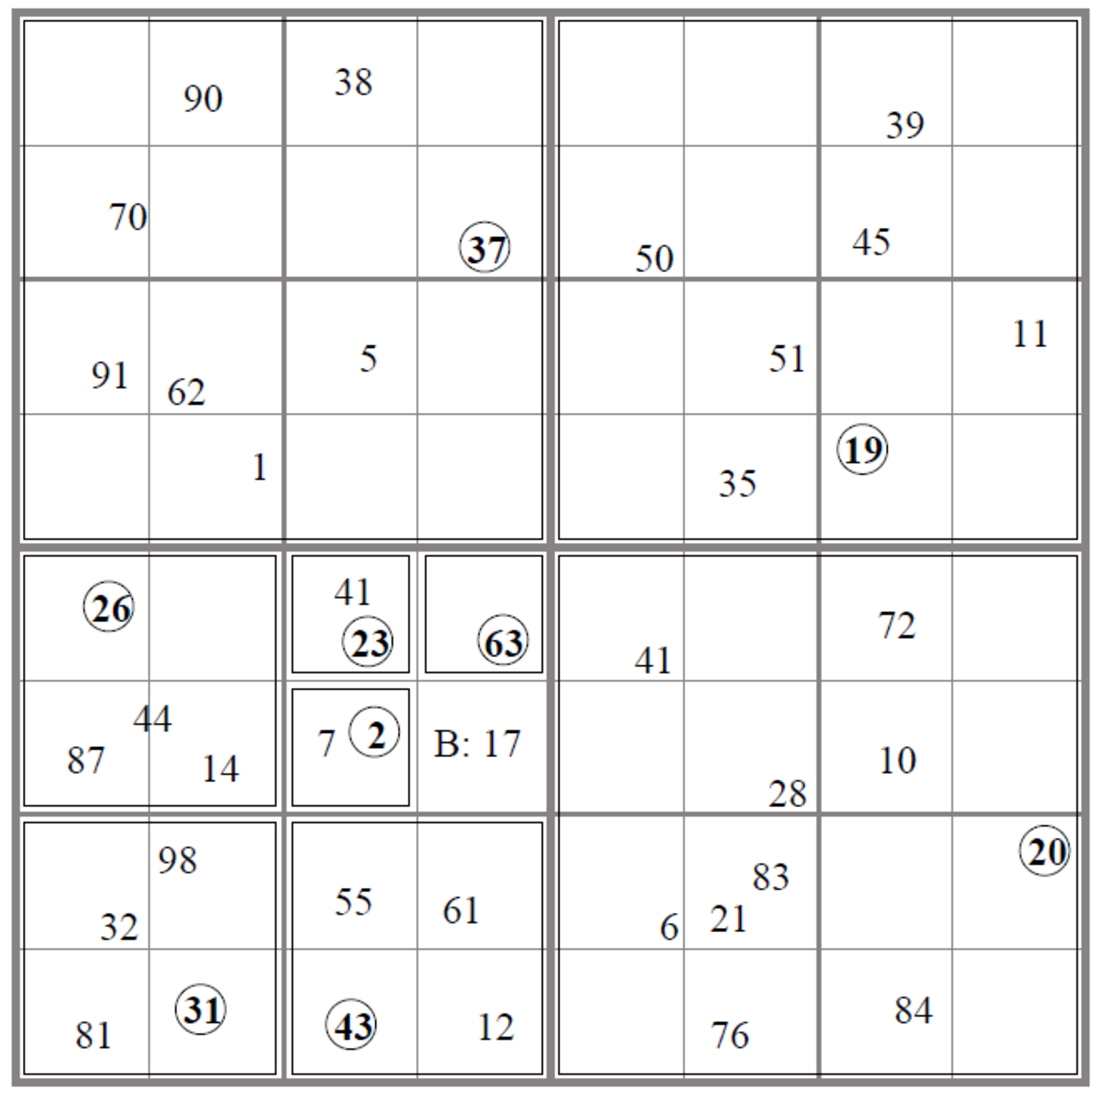
\includegraphics[width=\textwidth]{location_service}
\caption{Hierarchical grid with 4 order-i squares in order-i+1 square}
\end{figure}}
\end{column}
\end{columns}
\end{frame}


\begin{frame}{Location Service for GeoCRON}
\begin{columns}
\begin{column}{.5\textwidth}

	\begin{itemize}
		\item Grid $\Leftrightarrow$ CSN's \emph{geocells}
		\item Location servers $\rightarrow$ sensor's overlay contacts
		\item Natural geographic diversity $\rightarrow$ more robust!
		\item Location servers hold address, NOT just location!
		\item Region ID $\leftarrow$ quad tree path
		\vspace{-12pt} %strange formatting here, maybe the arrows?
		\begin{itemize}
			\item \emph{ex:} $B$ at 203 (count like Cartesian plane)
		\end{itemize}
		\item Region similarity $\rightarrow$ prefix match region ID
	\end{itemize}

\end{column}

\begin{column}{.5\textwidth}
\begin{figure}
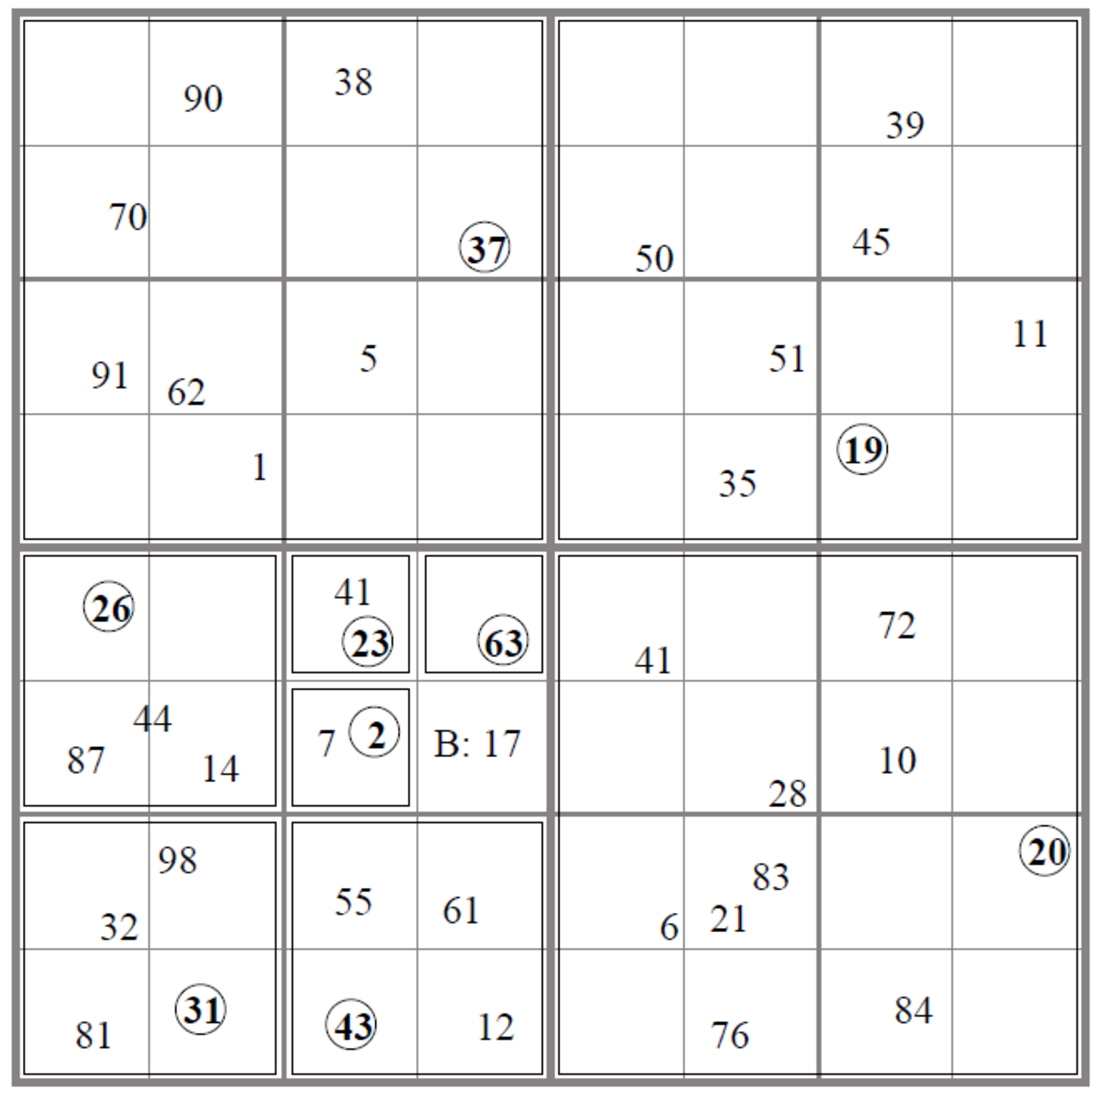
\includegraphics[width=\textwidth]{location_service}
\caption{Hierarchical grid closely resembles CSN's \emph{geocells}}
\end{figure}
\end{column}
\end{columns}
\end{frame}

% % % % % % % % % % % % % % % % % % % % % % % % % % % % % % % % % % % % % % % % % %

\section{Source Routing}

\begin{frame}{Source Routing}
	\begin{itemize}
		\item 
	\end{itemize}
\end{frame}

% % % % % % % % % % % % % % % % % % % % % % % % % % % % % % % % % % % % % % % % % %

\section{Greedy Forwarding}


\begin{frame}{Greedy Forwarding}
\begin{columns}
\begin{column}{.5\textwidth}
\begin{itemize}
	\item In \cite{749282}, source defines a \emph{multicast region} and \emph{forwarding zone}
		\begin{itemize}
			\item Message delivered to all nodes in multicast region
			\item Defined as a rectangle, coordinates inside message
			\item Includes source, destination, plus error
			\item Message flooded within forwarding zone until target reached
		\end{itemize}
\end{itemize}
\end{column}

\begin{column}{.5\textwidth}
\begin{figure}
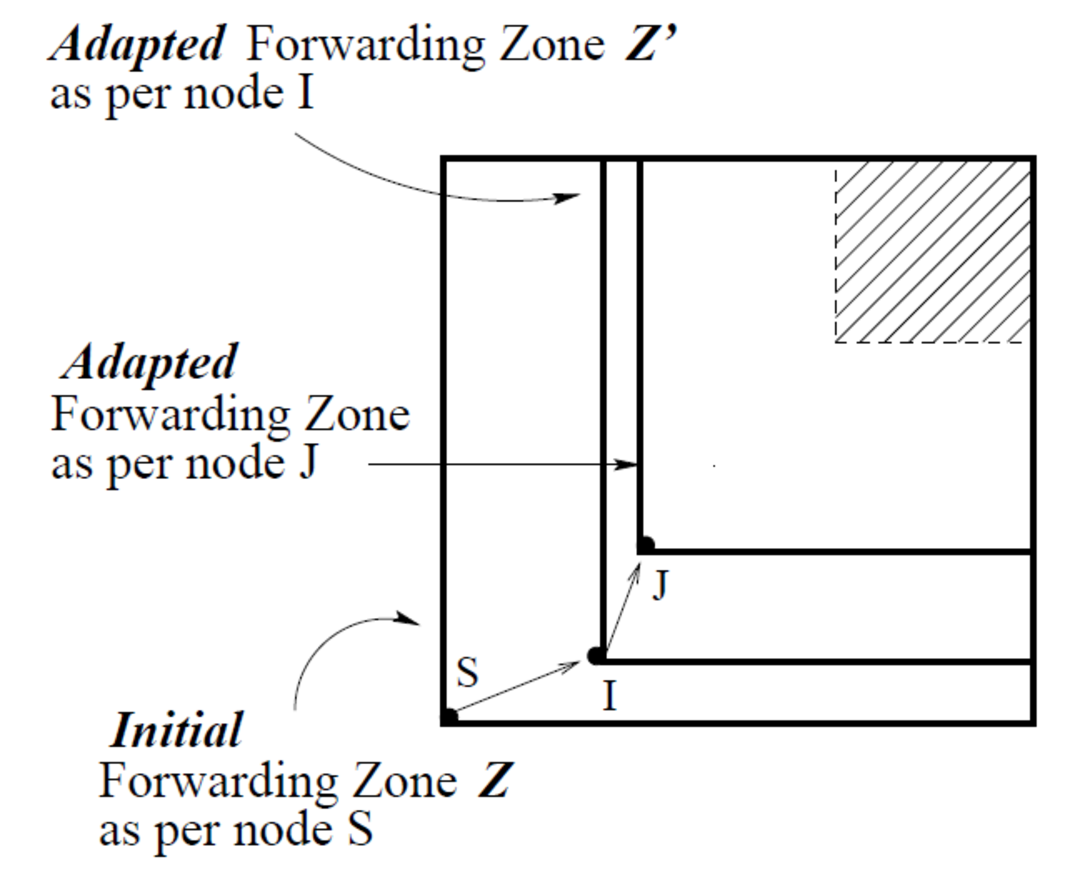
\includegraphics[width=\textwidth]{adaptive_geocast_region}
\caption{Depiction of adaptive multicast region and forwarding zone}
\end{figure}
\end{column}
\end{columns}
\end{frame}


\begin{frame}{Greedy Forwarding}
\begin{columns}
\begin{column}{.5\textwidth}
\begin{itemize}
	\item In \cite{749282}, source defines a \emph{multicast region} and \emph{forwarding zone}
		\begin{itemize}
			\item Message delivered to all nodes in multicast region
			\item Defined as a rectangle, coordinates inside message
			\item Includes source, destination, plus error
			\item Message flooded within forwarding zone until target reached
		\end{itemize}
\end{itemize}
\end{column}

\begin{column}{.5\textwidth}
\begin{figure}
\centering
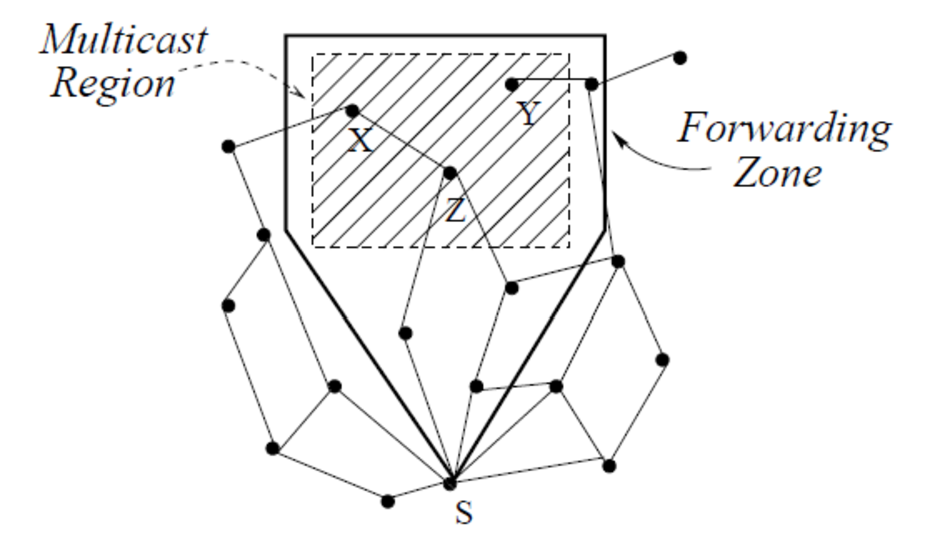
\includegraphics[width=\textwidth]{geocast_region}
\caption{Depiction of multicast region and forwarding zone}
\end{figure}
\end{column}
\end{columns}
\end{frame}


\begin{frame}{Greedy Forwarding}
\begin{columns}
\begin{column}{.5\textwidth}
\begin{itemize}
	\item Adapt forwarding region at each hop \cite{749282}
		\begin{itemize}
			\item Intermediate (closer) nodes know topology better
			\item Change region shape
		\end{itemize}
\end{itemize}
\end{column}

\begin{column}{.5\textwidth}
\begin{figure}
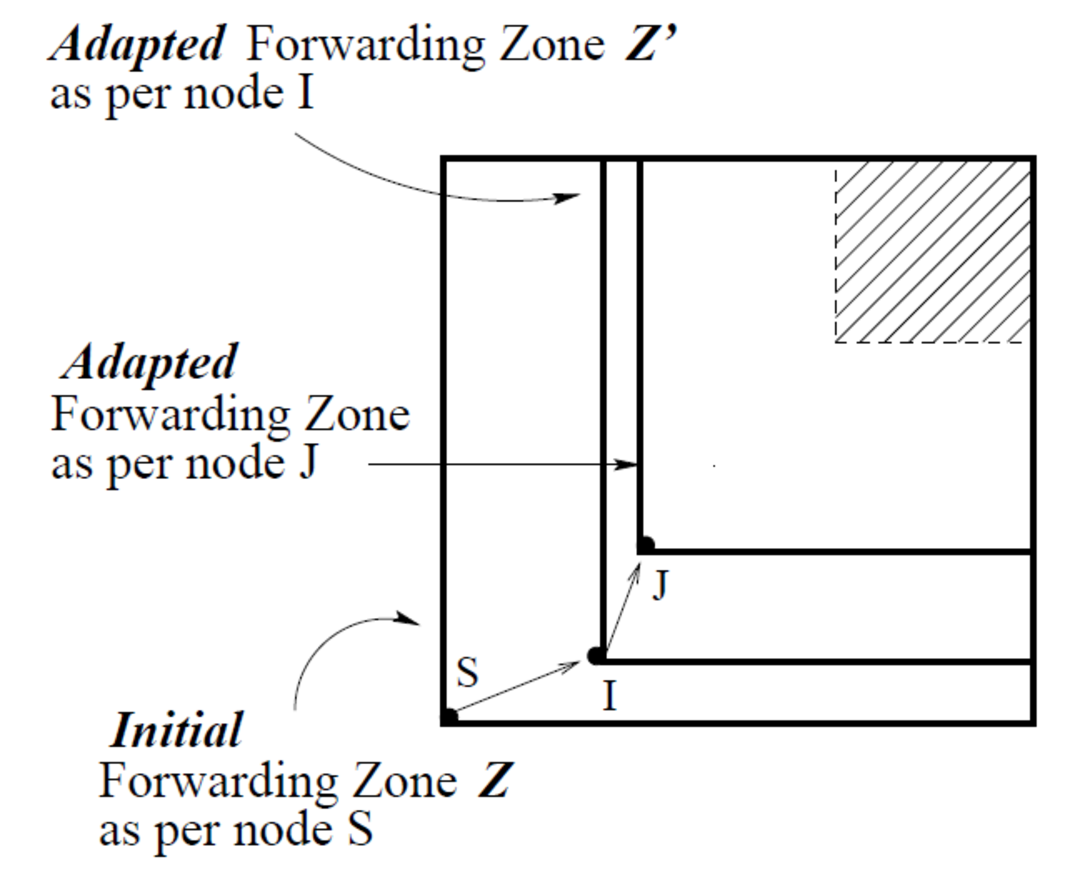
\includegraphics[width=\textwidth]{adaptive_geocast_region}
\caption{Depiction of adaptive multicast region and forwarding zone}
\end{figure}
\end{column}
\end{columns}
\end{frame}

% % % % % % % % % % % % % % % % % % % % % % % % % % % % % % % % % % % % % % % % % %

\section{Trajectory Routing}

% % % % % % % % % % % % % % % % % % % % % % % % % % % % % % % % % % % % % % % % % %

\section{Geometric Routing}

\begin{frame}{Geometric Routing}
	\begin{itemize}
		\item Network topology $\rightarrow$ graph
			\begin{itemize}
				\item Vertices $=$ nodes
				\item Edges $=$ direct communication
			\end{itemize}
		\pause
		\item Forward based on geometry of graph
		\pause
		\item \emph{Compass routing} first proposed in \cite{Kranakis99compassrouting}
		\begin{itemize}
			\item \emph{Right-hand rule}
			\begin{itemize}
				\item Forward packet along next counter-clockwise edge
				\item Analogous to following the right hand wall in a maze
			\end{itemize}
			\item Also called \emph{face routing}
			\item Also used in \cite{Kuhn2003}, ADD OTHERS HERE!!!!!!!!!!!!
		\end{itemize}
		\item 
	\end{itemize}
right-hand rule 
introduced in Compass Routing on Geometric Networks
\end{frame}

% % % % % % % % % % % % % % % % % % % % % % % % % % % % % % % % % % % % % % % % % %

\section{Clustering}

\begin{frame}
	
	In \cite{779923}, an inter-zone clustering protocol is periodically run to update with information about inter-zone links.
	Does not give information about exact location of destination within a zone and so still need to find that.
\end{frame}


\begin{frame}{Clustering - LABAR}
\begin{columns}
\begin{column}{.5\textwidth}
\begin{itemize}
	\item LABAR \cite{Zaruba2003}
		\begin{itemize}
			\item GPS-enabled nodes $\rightarrow$ backbone G-nodes
			\item Nodes near G-nodes belong to a \emph{zone}
			\item G-nodes give sender vector towards intermediary zones
		\end{itemize}
\end{itemize}
\end{column}

\begin{column}{.5\textwidth}
\begin{figure}
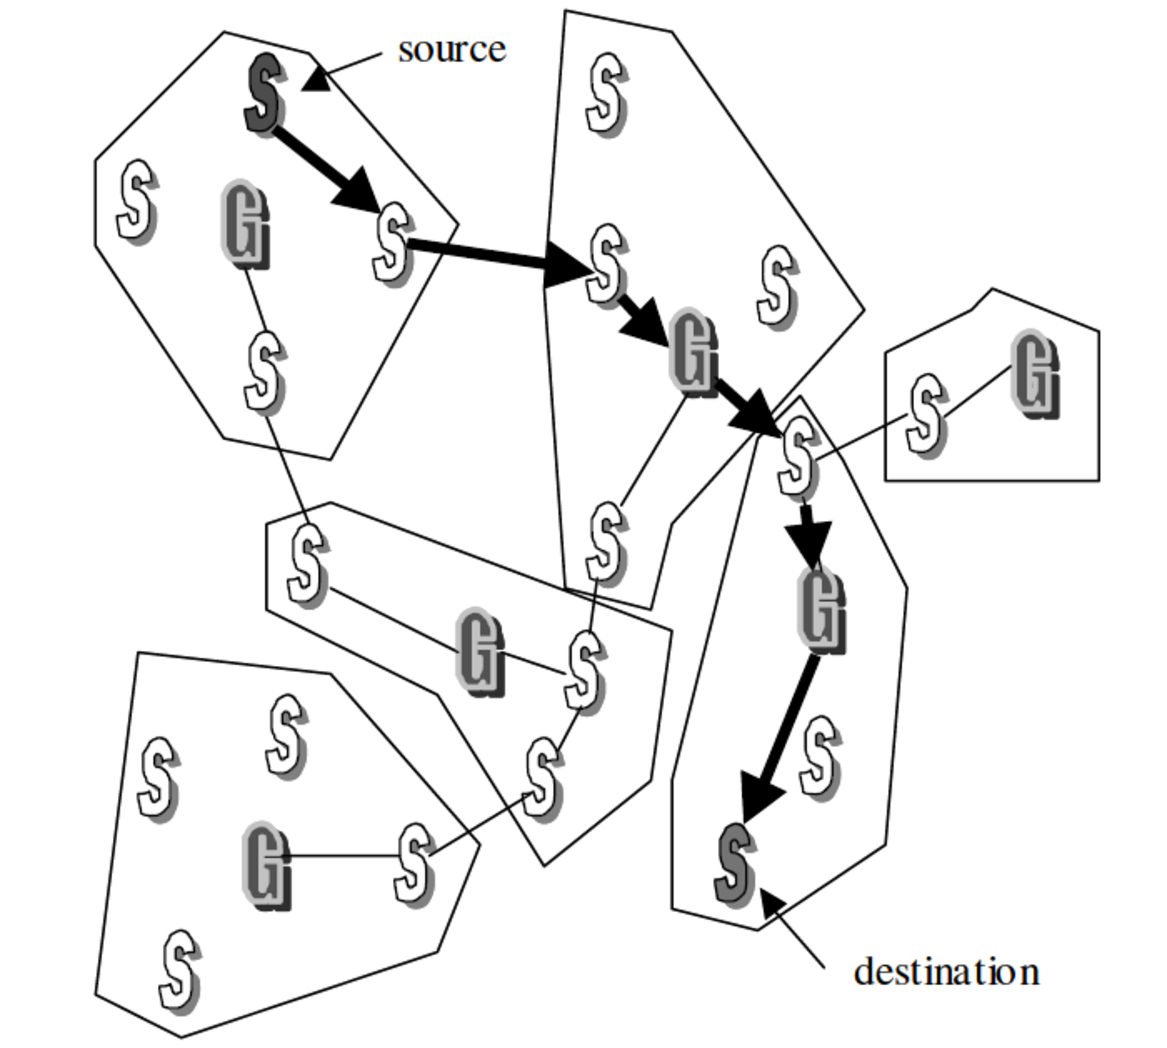
\includegraphics[width=\textwidth]{labar}
\caption{Routing in LABAR}
\end{figure}
\end{column}
\end{columns}
\end{frame}

% % % % % % % % % % % % % % % % % % % % % % % % % % % % % % % % % % % % % % % % % %

\section{Hybrid}

\begin{frame}{Hybrid}
\begin{itemize}
	\item In \cite{Kuhn2003, Huang2005, Karp2000}, greedy forwarding until \emph{void} reached
	\begin{itemize}
		\item \emph{Face routing} within a bounded region
		\item Enlarge bounded region if destination unreachable
		\item FAR \cite{Huang2005} introduced \emph{mobicast}: mobile geocast
		\begin{itemize}
			\item Application: mobile regional sensing
			\item \emph{Just in time} forwarding: packet arrives right before mobicast region
			\item Decreases \emph{lag time} (how long nodes hold data before mobicast region arrives)
		\end{itemize}
	\end{itemize}
\end{itemize}
\end{frame}

% % % % % % % % % % % % % % % % % % % % % % % % % % % % % % % % % % % % % % % % % %

\part{bib}

\begin{frame}{References}
\bibliographystyle{apalike}
% argument is your BibTeX string definitions and bibliography database(s)
\bibliography{IEEEabrv,location_routing}
\end{frame}

\end{document}
